\documentclass[tikz,border=10pt]{standalone}

\begin{document}
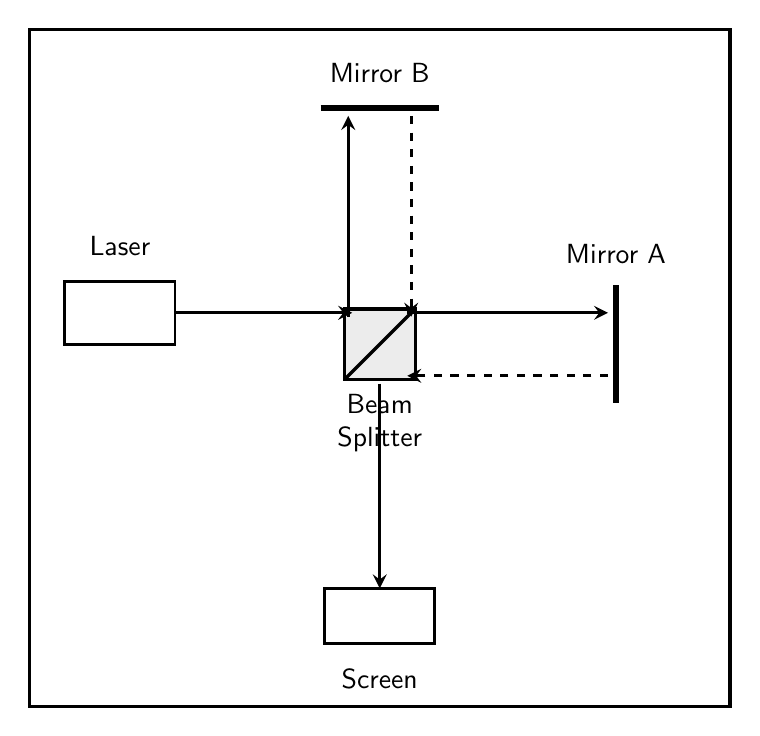
\begin{tikzpicture}[
  font=\sffamily,
  >=stealth,
  optical/.style={line width=1.2pt},
  beam/.style={->, line width=1.2pt},
  returnbeam/.style={->, line width=1.2pt, dashed},
  label/.style={align=center},
  mirror/.style={line width=2pt},
  device/.style={draw, line width=1pt, minimum width=1.4cm, minimum height=0.8cm}
]

\draw[device] (-4,0) rectangle (-2.6,0.8);
\node[label] at (-3.3,1.25) {Laser};

\draw[optical, fill=gray!15] (-0.45,-0.45) rectangle (0.45,0.45);
\draw[optical] (-0.45,-0.45) -- (0.45,0.45);
\node[label] at (0,-1.0) {Beam\\Splitter};

\draw[mirror] (3.0,0.75) -- (3.0,-0.75);
\node[label] at (3.0,1.15) {Mirror A};

\draw[mirror] (-0.75,3.0) -- (0.75,3.0);
\node[label] at (0,3.45) {Mirror B};

\draw[device] (-0.7,-3.8) rectangle (0.7,-3.1);
\node[label] at (0,-4.25) {Screen};

\draw[beam] (-2.6,0.4) -- (-0.35,0.4);
\draw[beam] (0.35,0.4) -- (2.9,0.4);
\draw[returnbeam] (2.9,-0.4) -- (0.35,-0.4);

\draw[beam] (-0.4,0.35) -- (-0.4,2.9);
\draw[returnbeam] (0.4,2.9) -- (0.4,0.35);

\draw[beam] (0.0,-0.5) -- (0.0,-3.1);

\draw[optical] (-4.45,-4.6) rectangle (4.45,4.0);

\end{tikzpicture}
\end{document}
